\documentclass[aspectratio=169,11pt]{beamer}
\def\courseweek{6}
% Shared style for the Introduction to Information Geometry lecture slides.
% Compile the lecture .tex files from this directory.
\providecommand{\courseweek}{1}
\usepackage[T1]{fontenc}
\usepackage[utf8]{inputenc}
\usepackage[sc]{mathpazo}
\renewcommand{\sfdefault}{lmss}
\renewcommand{\ttdefault}{lmtt}
\usepackage{amsmath,amssymb,mathtools}
\usepackage{tikz}
\usetikzlibrary{arrows.meta,calc,positioning}
\usepackage{pgfplots}
\pgfplotsset{compat=1.18}
\usepackage{booktabs}

\definecolor{courseink}{HTML}{173749}
\definecolor{coursemuted}{HTML}{526674}
\definecolor{courseteal}{HTML}{0E7287}
\definecolor{coursecopper}{HTML}{B66B43}
\definecolor{courseline}{HTML}{D4E0E3}
\definecolor{coursepale}{HTML}{EFF5F5}

\setbeamercolor{normal text}{fg=courseink,bg=white}
\setbeamercolor{structure}{fg=courseteal}
\setbeamercolor{frametitle}{fg=courseink,bg=white}
\setbeamercolor{title}{fg=courseink}
\setbeamercolor{subtitle}{fg=coursemuted}
\setbeamercolor{block title}{fg=courseink,bg=white}
\setbeamercolor{block body}{fg=courseink,bg=white}
\setbeamercolor{alerted text}{fg=coursecopper}
\setbeamerfont{title}{family=\rmfamily,series=\bfseries,size=\fontsize{32}{37}}
\setbeamerfont{frametitle}{family=\rmfamily,series=\bfseries,size=\fontsize{26}{31}}
\setbeamerfont{normal text}{size=\fontsize{18}{22}}
\setbeamerfont{subtitle}{size=\fontsize{17}{21}}
\setbeamersize{text margin left=0.78cm,text margin right=0.78cm}
\setbeamertemplate{navigation symbols}{}
\setbeamertemplate{itemize items}[circle]
\setbeamertemplate{enumerate items}[default]
\setbeamertemplate{blocks}[default]
\setlength{\parskip}{0.22em}
\setbeamertemplate{footline}{%
  \leavevmode\hbox to \paperwidth{\hspace{.78cm}%
  {\color{coursemuted}\fontsize{8.5}{10}\selectfont Introduction to Information Geometry \hspace{.32cm} / \hspace{.32cm} Week \courseweek}%
  \hfill{\color{coursemuted}\fontsize{8.5}{10}\selectfont \insertframenumber\hspace{.17cm}/\hspace{.17cm}\inserttotalframenumber}\hspace{.78cm}}%
  \vskip.17cm
}
\setbeamertemplate{frametitle}{%
  \vspace{.13cm}
  \insertframetitle\par
  \vspace{.08cm}
}
\setbeamertemplate{title page}{%
  \vspace*{1.00cm}
  {\color{courseteal}\fontsize{10}{13}\selectfont\bfseries
  INTRODUCTION TO INFORMATION GEOMETRY\par}
  \vspace{.40cm}
  {\usebeamerfont{title}\usebeamercolor[fg]{title}\inserttitle\par}
  \vspace{.22cm}
  {\usebeamerfont{subtitle}\usebeamercolor[fg]{subtitle}\insertsubtitle\par}
  \vfill
  {\color{coursemuted}\fontsize{13}{16}\selectfont Christopher Lee\par}
  \vspace{.34cm}
}

\pgfplotsset{
  courseplot/.style={
    width=11.05cm,
    height=5.15cm,
    axis line style={coursemuted!75},
    tick style={coursemuted!65},
    ticklabel style={font=\scriptsize,color=coursemuted},
    label style={font=\normalsize,color=courseink},
    grid=major,
    major grid style={courseline!70,line width=.4pt},
    line width=1.45pt,
    legend style={font=\small,draw=none,fill=none,at={(.98,.03)},anchor=south east},
    clip=true
  }
}

\newcommand{\highlightmath}[1]{{\color{courseteal}#1}}
\newcommand{\thinrule}{\par\vspace{.25cm}{\color{courseline}\rule{\linewidth}{.8pt}}\par}

% A one-dimensional state space.  x=0 and x=1 are placed at 0 and 9 units.
\newcommand{\stateinterval}[1]{%
 \begin{tikzpicture}[x=1cm,y=1cm]
   \draw[courseink,line width=1.25pt] (0,0)--(9,0);
   \foreach \pos/\lab in {0/0,9/1} {
     \fill[courseink] (\pos,0) circle(2.7pt);
     \node[below=9pt,text=coursemuted] at (\pos,0) {\(\lab\)};
   }
   #1
 \end{tikzpicture}%
}

% Paired pages are separate frames in the PDF, with matching titles.
% Supply the whole frame body for each version; the instructor may edit them
% independently without changing overlay logic.
\newcommand{\coursepair}[3]{%
  \begin{frame}{#1}#2\end{frame}%
  \begin{frame}{#1}#3\end{frame}%
}

% Equilateral representation of the categorical simplex, in barycentric
% coordinates with vertices A=(0,0), B=(1,0), C=(1/2,sqrt(3)/2).
\newcommand{\coursesimplex}[1]{%
 \begin{tikzpicture}[scale=4.9]
  \fill[coursepale] (0,0)--(1,0)--(.5,.8660254)--cycle;
  \draw[courseink,line width=.65pt] (0,0)--(1,0)--(.5,.8660254)--cycle;
  \node[below left,font=\small] at (0,0) {A};
  \node[below right,font=\small] at (1,0) {B};
  \node[above,font=\small] at (.5,.8660254) {C};
  #1
 \end{tikzpicture}%
}

\title{Relative Entropy as a Lyapunov Function}
\subtitle{Week 6 \(\cdot\) Lecture 2}
\date{}
\begin{document}
\begin{frame}[plain]\titlepage\end{frame}

\begin{frame}{A scalar function can monitor a flow}
For \(x'=F(x)\), a Lyapunov function \(V(x)\) has
a strict minimum at an equilibrium \(q\).
\vspace{.48cm}
If
\[
\highlightmath{\dot V(x)=V'(x)F(x)\leq0},
\]
\vspace{.34cm}
its value cannot increase along trajectories.
When the derivative is strictly negative away from \(q\),
the function can establish attraction.
\end{frame}

\begin{frame}{KL divergence from an equilibrium law}
For a two-type law, fix \(q\in(0,1)\) and define
\[
\highlightmath{V(x)=D(q\|x)}
\]
\vspace{.25cm}
\[
=q\ln\frac qx+(1-q)\ln\frac{1-q}{1-x}.
\]
\vspace{.46cm}
Its minimum is at \(x=q\), where \(V(q)=0\).
\end{frame}

\begin{frame}{The key derivative}
Differentiate with respect to the evolving coordinate \(x\):
\[
\begin{aligned}
V'(x)&=-\frac qx+\frac{1-q}{1-x}\\[4pt]
&=\highlightmath{\frac{x-q}{x(1-x)}}.
\end{aligned}
\]
\vspace{.50cm}
The denominator will cancel the replicator factor \(x(1-x)\).
\end{frame}

\coursepair{A global stability calculation}{
Consider \(x'=x(1-x)(3-4x)\) with \(q=\frac34\).
\vspace{.40cm}
Let \(V(x)=D(q\|x)\). Using
\[
V'(x)=\frac{x-q}{x(1-x)},
\]
find \(\dot V=V'(x)x'\).
}{
Consider \(x'=x(1-x)(3-4x)\) with \(q=\frac34\).
\vspace{.40cm}
The factors cancel:
\[
\dot V=(x-\tfrac34)(3-4x)
=\highlightmath{-4(x-\tfrac34)^2}.
\]
\vspace{.25cm}
It is negative at every non-equilibrium interior state.
}

\begin{frame}{Relative entropy is a bowl around the target}
\vspace{-.25cm}
\begin{center}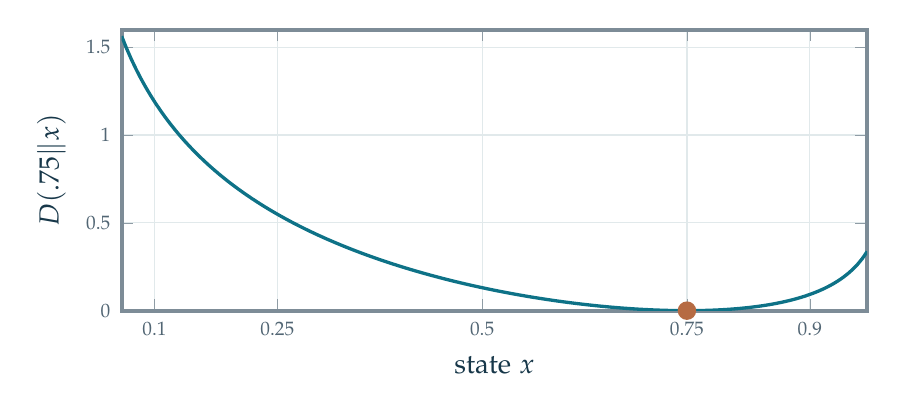
\begin{tikzpicture}
\begin{axis}[courseplot,xmin=.06,xmax=.97,ymin=0,ymax=1.6,
 xlabel={state $x$},ylabel={$D(.75\|x)$},xtick={.1,.25,.5,.75,.9},
 ytick={0,.5,1,1.5}]
\addplot[courseteal,very thick,domain=.06:.97,samples=155]
{.75*ln(.75/x)+.25*ln(.25/(1-x))};
\addplot[only marks,coursecopper,mark=*,mark size=2.6pt]coordinates{(.75,0)};
\end{axis}\end{tikzpicture}\end{center}
\vspace{-.12cm}
Its sublevel intervals remain away from \(0\) and \(1\).
\end{frame}

\begin{frame}{A global conclusion from local information}
For \(x'=x(1-x)(a-bx)\) with \(b>0\) and \(q=a/b\in(0,1)\),
\[
\highlightmath{\frac d{dt}D(q\|x)=-b(x-q)^2}.
\]
\vspace{.5cm}
Because KL diverges at both endpoints, its finite sublevel sets
are compact inside \((0,1)\).
\vspace{.34cm}
Every interior trajectory approaches \(q\).
\end{frame}

\begin{frame}{Many strategies: a short formula}
Let \(\mathbf q\) be a fixed positive reference law and
\(p_i'=p_i(f_i-\bar f)\).
\vspace{.40cm}
Differentiate \(D(\mathbf q\|\mathbf p(t))\):
\[
\begin{aligned}
\frac d{dt}D(\mathbf q\|\mathbf p)
&=-\sum_iq_i\frac{p_i'}{p_i}\\[4pt]
&=\highlightmath{\bar f-\sum_iq_if_i}.
\end{aligned}
\]
\end{frame}

\coursepair{The cyclic family revisited}{
For the cyclic family, let \(\mathbf q=(\frac13,\frac13,\frac13)\)
and \(P=p_Ap_Bp_C\).
\vspace{.33cm}
We know
\[
D(\mathbf q\|\mathbf p)=-\frac13\ln(27P),
\qquad \frac d{dt}\ln P=(1-s)(1-3Q).
\]
\vspace{.30cm}
Find \(\frac d{dt}D(\mathbf q\|\mathbf p)\).
}{
For the cyclic family, let \(\mathbf q=(\frac13,\frac13,\frac13)\)
and \(P=p_Ap_Bp_C\).
\vspace{.33cm}
The KL derivative is
\[
\highlightmath{\frac d{dt}D(\mathbf q\|\mathbf p)
=-\frac{1-s}{3}(1-3Q)}.
\]
\vspace{.3cm}
It decays for \(s<1\), is constant for \(s=1\), and increases for \(s>1\).
}

\begin{frame}{The quadratic approximation of KL}
For a Bernoulli reference \(q\) and a small displacement \(u\),
\[
\highlightmath{D(q\|q+u)=\frac{u^2}{2q(1-q)}+O(u^3)}.
\]
\vspace{.48cm}
The coefficient depends on the reference distribution.
An equal coordinate change can have a different information cost
at a different state.
\end{frame}

\coursepair{Two equal changes with unequal costs}{
Use \(u=0.01\) in the quadratic KL approximation
\[
D(q\|q+u)\approx\frac{u^2}{2q(1-q)}.
\]
\vspace{.42cm}
Compare \(q=0.2\) with \(q=0.5\).
}{
Use \(u=0.01\) in the quadratic KL approximation
\[
D(q\|q+u)\approx\frac{u^2}{2q(1-q)}.
\]
\vspace{.42cm}
At \(q=0.2\), the cost is \(\highlightmath{0.0003125}\).
At \(q=0.5\), it is \(\highlightmath{0.0002}\).
}

\begin{frame}{A quadratic form on the simplex}
For an interior reference law \(\mathbf q\) and tangent displacement
\(\mathbf u\) with \(\sum_i u_i=0\),
\[
\highlightmath{D(\mathbf q\|\mathbf q+\mathbf u)
=\frac12\sum_i\frac{u_i^2}{q_i}+O(\|\mathbf u\|^3)}.
\]
\vspace{.52cm}
The quadratic term defines a state-dependent inner product
on the tangent space. That is the Fisher information metric.
\end{frame}
\end{document}
